\documentclass[utf8]{article}

\usepackage[utf8]{inputenc}

\usepackage[parfill]{parskip}

\usepackage{amsmath}
\usepackage{mathtools}
\usepackage{nccmath}
\usepackage{amssymb}
\usepackage{amsfonts}
\usepackage{graphicx}
\usepackage{float}
\usepackage{listingsutf8}
\usepackage{hyperref}
\usepackage[dvipsnames]{xcolor}
\usepackage{comment}

\usepackage{fullpage}

%------------------------------------------------------

\usepackage{listings}

\definecolor{color0}{RGB}{147, 147, 147}
\definecolor{color1}{RGB}{186, 033, 033}
\definecolor{color2}{RGB}{000, 128, 000}
\definecolor{color3}{RGB}{064, 128, 128}
\definecolor{color4}{RGB}{170, 034, 255}

\lstdefinelanguage{clips}{
  mathescape = true,
  sensitive        = true,
  morecomment      = [l]{;},
  showstringspaces = false,
  morestring       = [b]",
}

% egreg's modulo macro (see https://tex.stackexchange.com/a/34449/21891)
\def\truncdiv#1#2{((#1-(#2-1)/2)/#2)}
\def\moduloop#1#2{(#1-\truncdiv{#1}{#2}*#2)}
\def\modulo#1#2{\number\numexpr\moduloop{#1}{#2}\relax}


\makeatletter

% a TeX counter to keep track of the nesting level
\newcount\netParensCount@clisp

% Modify how ( and ) get typeset depending on the value of the counter
% (Based on Ulrike Fischer's approach to modifying characters in listings;
% see https://tex.stackexchange.com/a/231927/21891)
\lst@CCPutMacro
\lst@ProcessOther{`(}{{%
  \ifnum\lst@mode=\lst@Pmode\relax%
    \rainbow@clisp{(}%
    \global\advance\netParensCount@clisp by \@ne%
  \else
    (%
  \fi
}}%
\lst@ProcessOther{`)}{{%
  \ifnum\lst@mode=\lst@Pmode\relax%
    \global\advance\netParensCount@clisp by \m@ne%
    \rainbow@clisp{)}%
  \else
    )%
  \fi
}}%
\@empty\z@\@empty

% Color its argument based on the value of the \netParensCount@clisp counter
% (modulo 5)
\newcommand\rainbow@clisp[1]{%
  \ifcase\modulo\netParensCount@clisp 5\relax%
    \textcolor{color0}{#1}%
  \or
    \textcolor{color1}{#1}%
  \or
    \textcolor{color2}{#1}%
  \or
    \textcolor{color3}{#1}%
  \else
    \textcolor{color4}{#1}%
  \fi
}

\lst@AddToHook{PreInit}{%
  \global\netParensCount@clisp 0\relax%
}

\makeatother

\lstnewenvironment{clips-code}
  {\lstset{language=clips}}
  {}

\setcounter{tocdepth}{6}
\setcounter{secnumdepth}{6}

% -----------------------------------------------------


\title{INFO-F-305 - Modélisation et Simulation
\\Projet Octave
\\Wall-e}
\author{Becker Robin Gilles - Bourgeois Noé}
\date{December 2022}

\begin{document}
\maketitle
\tableofcontents

\newpage

% -----------------------------------------------------

\section{Introduction}

\section{Modélisation}
\section{Analyse de cas}
\subsection{Les sentiments d’EVE ne dépendent pas de WALL-E}

\begin{equation}
\centering
\left\{\begin{split}
\dot{w}(t) &= aw(t) + be(t)\\
\dot{e}(t) &= 0 \\
\end{split}\right.
 \end{equation}

\subsection{Les deux robots ont la même dynamique}

\begin{equation}
\centering
\left\{\begin{split}
\dot{w}(t) &= aw(t) + be(t)\\
\dot{e}(t) &= bw(t) + ae(t) \\
\end{split}\right.
 \end{equation}

On peut en déduire la matrice à coefficients A telle que X˙ (t) = Ax :

% coefficients matrix A
\begin{equation}
\centering
A = \left[
\begin{array}{cc}
a & b\\
b & a
\end{array}
\right]
 \end{equation}

De là, nous pouvons décider d’utliser le diagramme de Pointcarré
ou la méthode des valeurs propres
pour définir le type de système (selle, nœud stable, ….)
Dans cet exemple, nous allons utiliser
les valeurs propres.
On calcule les valeurs propres en posant l’équation caractéristique :

\begin{equation}
\centering
\det(A − λI) = 0
 \end{equation}

On résoud et on obtient les valeurs propres :

\begin{equation}
\centering
\lambda_1,2 = 2a \pm \sqrt{4b^2} = {a - b, a + b}
 \end{equation}

On distingue les différents cas possibles :
1. Selle : pour que le système soit une selle, il faut
λ1,2 ̸= 0
et
signe(λ1) ̸= signe(λ2). On a

% display graph
\begin{figure}[h]
\centering
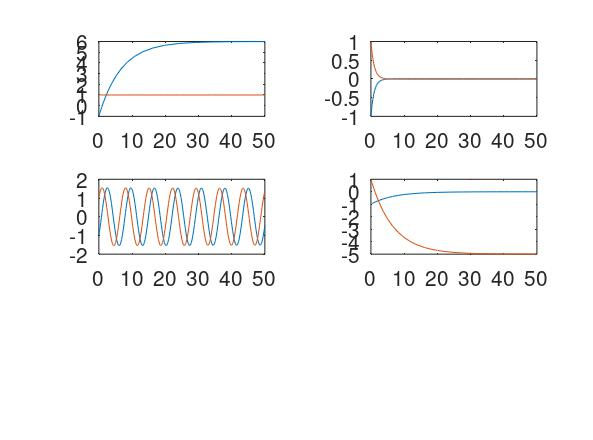
\includegraphics[width=0.5\textwidth]{pics/graphs}
\caption{Selle}
\end{figure}

\subsection{Les deux robots auront une dynamique contrastante}

3. Les deux robots auront une dynamique contrastante :

\begin{equation}
\centering
\left\{\begin{split}
\dot{w}(t) &= aw(t) + be(t)\\
\dot{e}(t) &= −bw(t) − ae(t) \\
\end{split}\right.
 \end{equation}


\subsection{La dynamique de chaque robot dépend simplement de l’autre
robot}

\begin{equation}
\centering
\left\{\begin{split}
\dot{w}(t) &= aw(t) + be(t)\\
\dot{e}(t) &= −bw(t) − ae(t) \\
\end{split}\right.
 \end{equation}

\subsection{Bonus : a n’est pas une constante mais dépend du temps}

On pose a(t) = max(0, 100 − 0.1t).

\begin{equation}
\centering
\left\{\begin{split}
\dot{w}(t) &= a(t)w(t) + be(t)\\
\dot{e}(t) &= bw(t) + a(t)e(t) \\
\end{split}\right.
 \end{equation}



\section{Conclusion}
Nous

\end{document}
